\section{Experimental results}
\label{sec:exp}

The experiments follow a mission similar to the original plan given in
Fig. \ref{fig:ex:plan}. At the beginning, the AUV need to {\em Sample
  Vent2} and it has to return to the {\em surface} by the end of the
mission. The AUV must also be at the {\em surface} around the time 13:00. We
implemented this on our executive with plans being produced by the
europa planning engine \cite{frank2003}. Figure \ref{fig:ex:mixed1} 
demonstrates the resulting plan after processing from 
Algorithm \ref{alg:dispatch}.

\begin{figure}[!htbp]
  \centering
  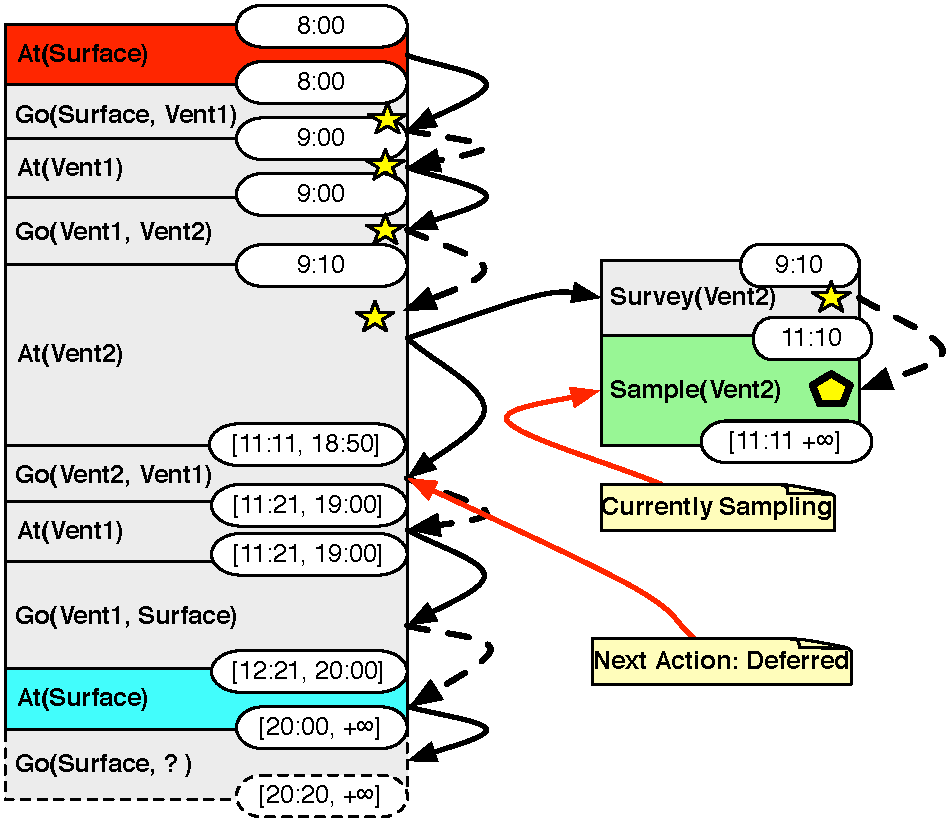
\includegraphics[width=0.8\columnwidth]{figs/example_MixedInitial}
  \caption{\small The algorithmic solution for the plan from
    Fig. \ref{fig:ex:plan}. Solid lines indicate conditions and
    dashed lines indicate effects. Pentagons indicate {\em urgent}
    goals, stars indicate tokens that were deduced as {\em proactive}.}
  \label{fig:ex:mixed1}
\end{figure}

For Algorithm \ref{SearchForGoal}, the search is straight forward. For
example in Fig. \ref{fig:ex:mixed1}, if the AUV is {\em At Surface} then
the next {\em Go} token will be dispatched. Because the search will
follow the causal links forward, where upon, it will find the goal
{\em Sample Vent2} resulting in dispatching proactively.  Similarly,
this occurs for all of the tokens that are starred. The next token that is
not starred, {\em Go(Surface)}, is continuously searched but deferred,
because it is not connected to an urgent goal. The resulting AUV stays 
at {\em Vent2} rather than heading to the {\em Surface} immediately.

%For the distributed algorithm approach, each token is checked during
%the creation of the plan to see if it is an external goal in
%$\Phi_{ge}$, or connected to one through a causal link. When the {\em
%Sample Vent2} is checked, we immediately find that it is a goal. We then
%follow the reverse causal link and find {\em Survey Vent2}.  However to
%better illustrate the algorithm, we can imagine that only the {\em Survey
%Vent2} has been causally connected to the goal so far. Therefore, we
%only star those two tokens. The path from {\em Surface} to {\em Vent1}
%to {\em Vent2} has yet to be built. When the path has finally been
%built, and {\em At Vent2} is checked, our algorithm searches one
%causal link and finds {\em Survey Vent2} which is starred. The search
%then follows the reverse causal link and stars the rest of the
%path. The starred tokens will then be proactively dispatched while the
%non-starred tokens will be deferred until later. Having similar
%results to Algorithm \ref{DispatchToken}.

\begin{figure}[!htbp]
  \centering
  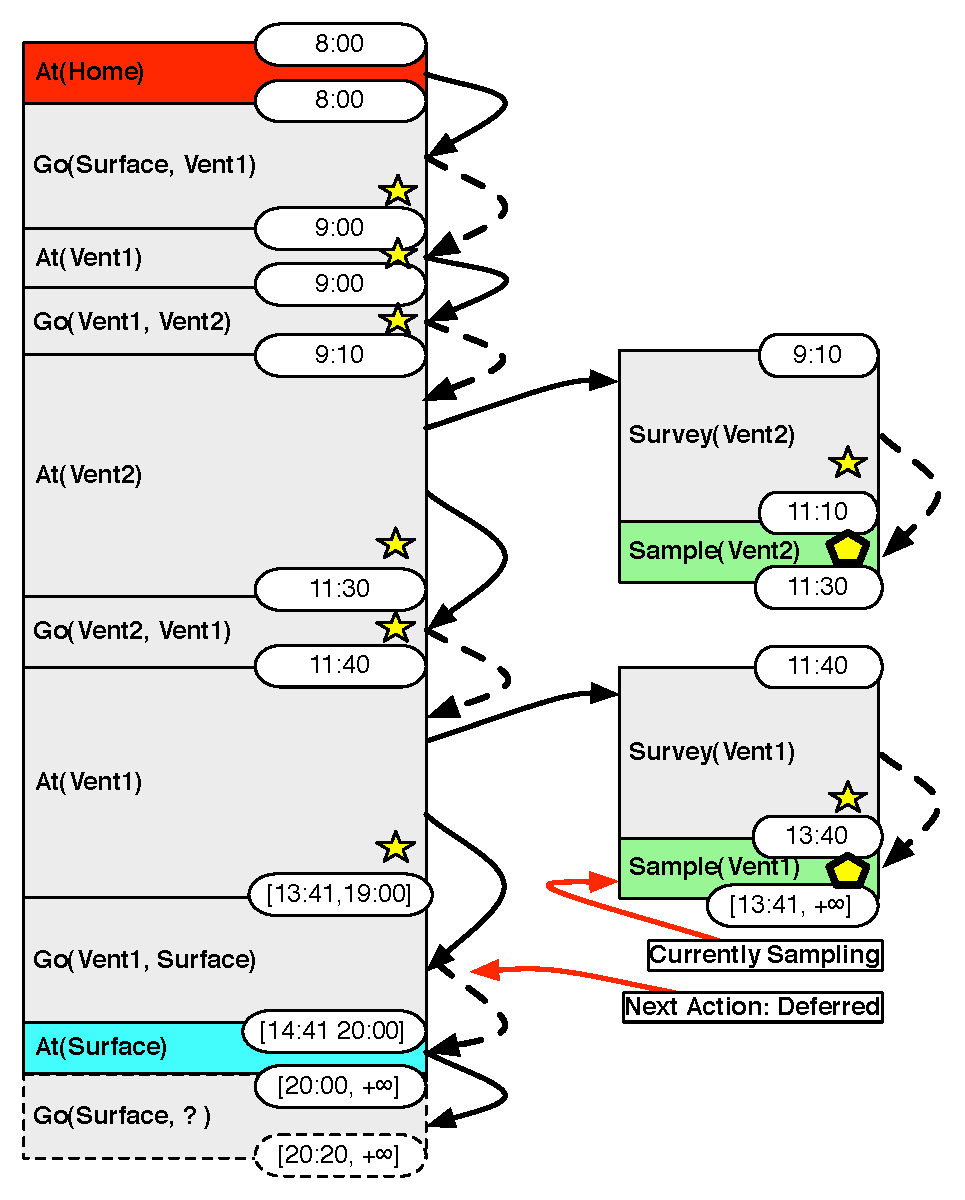
\includegraphics[width=0.8\columnwidth]{figs/example_MixedUpdate}
  \caption{\small The solution after receiving external request for
    the plan from Fig. \ref{fig:ex:mixed1}}
  \label{fig:ex:mixed2}
\end{figure}

In this run we then introduced a new {\em urgent} goal to {\em Sample
Vent1} at 11:30. We show the resulting plan in
Fig. \ref{fig:ex:mixed2}. There is not enough
time to {\em Sample Vent1} and be at the surface by 13:00. Therefore,
the goal is placed after the AUV goes to the surface. As a result the
actions which were so fdfar marked as deferred are now also causaly
linked to the new {\em urgent} goal. Therefore their former execution
policy is now updated. The resulting starred tokens in
Fig. \ref{fig:ex:mixed2} get dispatched proactively and includes all
the actions related to this mid-day surfacing goal.

Meanwhile the actions related to the last surfacing goal remains {\em
  deferred} and won't be executed until 19:00 allowing the vehicle to
sample {\em Vent1} for a duration of 2:50 hours.  After returning to the {\em
  Surface}, our planner and domain inserted a  partially instantiated
action to {\em Go(Surface, ?)} (dashed in the figures). 
This is an artifact resulting from the plan model which specifies that 
an {\em At} token is necessarily followed by a {\em Go}.
However, our algorithm will not be dispatching this token as it is not
connected to an {\em urgent} goal and its upper bound 
start time ($+\infty$) will not be met within the scope of the
mission. 

\begin{figure}[!htbp]
  \centering
  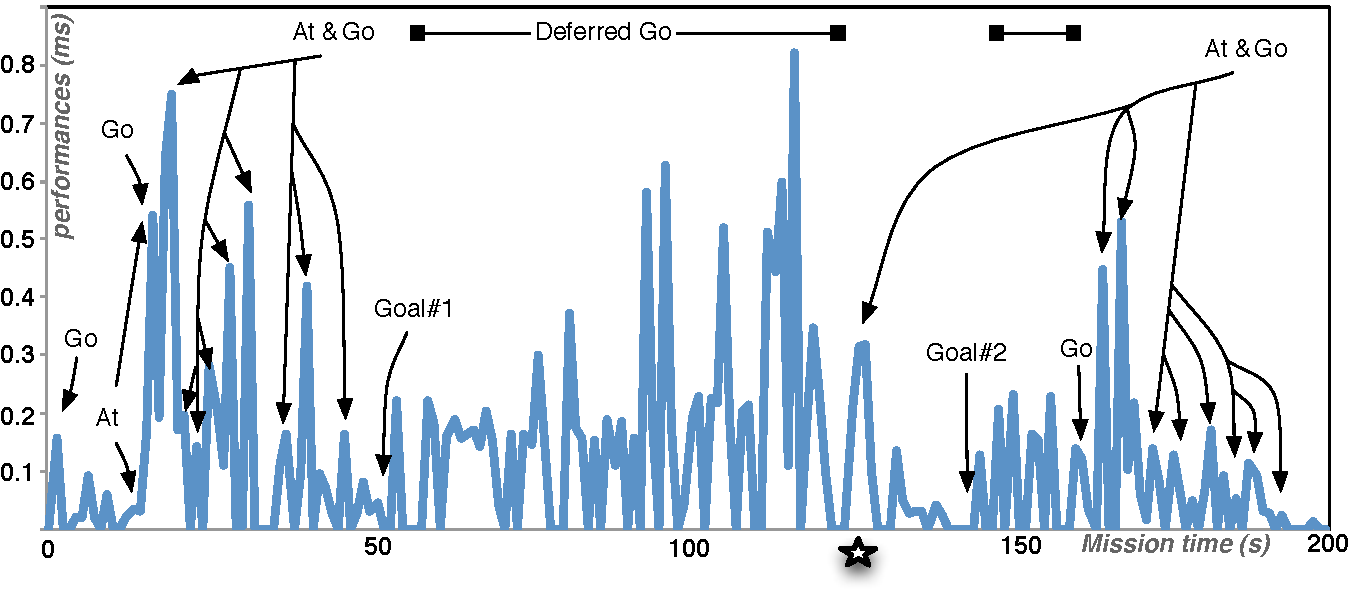
\includegraphics[width=\columnwidth]{figs/example_run.pdf}
  \caption{\small One mission run that shows the time needed for
    dispatching. The star represents when the Goal\#2 was received and
    integrated into the plan. Lines with boxes at the end represent
    the deferred action {\em Go} Because of space, we didn't put an
    arrow to every {\em At}. Our concern were the peaks that showed
    where the system had to dispatch both {\em At} and {\em Go}. }
  \label{fig:example_run}
\end{figure}


In our experiments, the simulated AUV missions ran in a virtual
machine running Ubuntu, a Linux distribution. The virtual machine was
run on a MacBook Pro and was allocated one core from
a $2.33$ GHz Intel Core $2$ Duo processor. Time was
recorded using a thread clock for the most accurate time. The length of
the mission was roughly 200 seconds. This was meant to allow many
simulations to be completed quickly. There is, however, no difference in 
performance if the mission were longer as the same plan would be produced
just with different times.

Figure \ref{fig:example_run} shows a simulated mission run that
is similar to the original example in Fig. \ref{fig:ex:plan}.
However, in order to increase the complexity of the plan a
total of eight locations were added before the vents. The first goal is to
{\em Sample vent2} at location ten and the second is to {\em Sample
  vent1} at location nine. The spikes in the time happen when it
dispatches both an {\em At} and a {\em Go} token which means that the graph
was searched twice. There is a clear trend that as the AUV gets
closer to the goals the time decreases because the search distance
decreases.  However, there is some variability in the time which can
most likely be accounted for as time added by context switching as the
virtual machine only had one processor. Before Goal\#2 is integrated
into the plan at time $127$, the algorithm is continually searching the
graph from the next {\em Go}, from time $54$ through $126$. The time is on an average above $.2$
milliseconds as the search is exhaustive. At tick $127$, the {\em Go} is no longer deferred and gets
dispatched quickly. The search for Goal\#2 becomes relatively simple as it is
not very far away in the plan, and thus the time decreases
significantly.

\begin{figure}[!htbp]
  \centering
  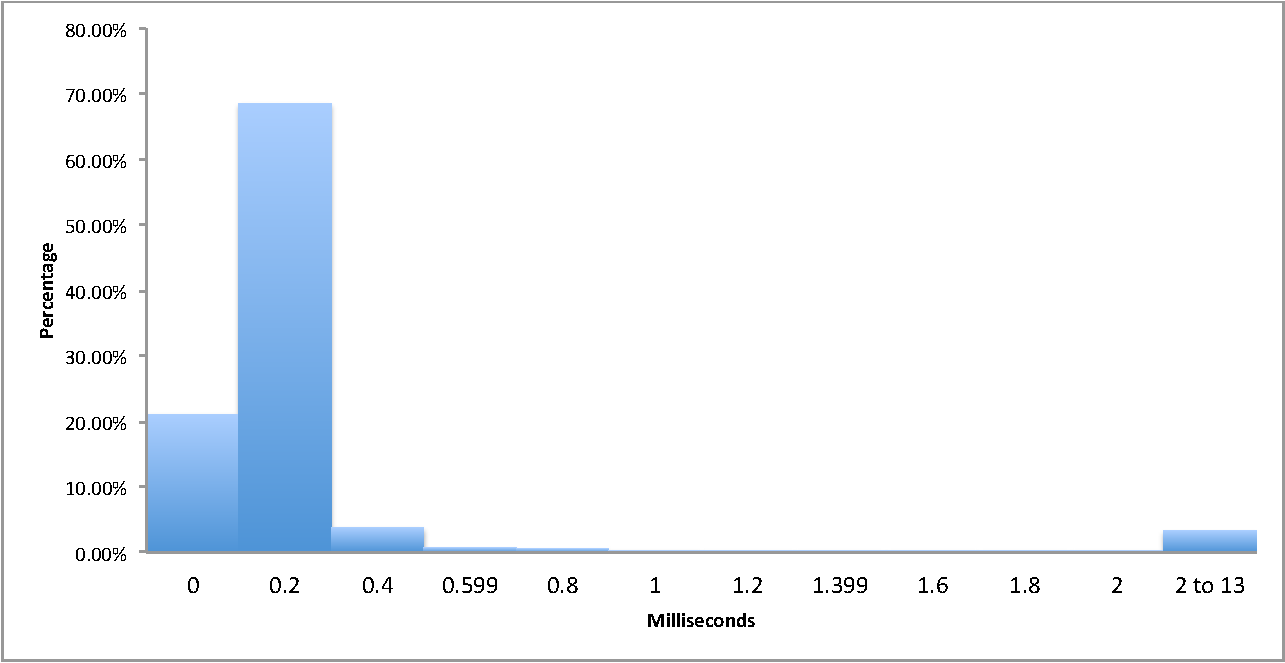
\includegraphics[width=\columnwidth]{figs/HistogramAlg1}
  \caption{\small Algorithm \ref{DispatchToken} was 
  timed at every increment of the mission time for $500$ 
  simulated missions. One goal was inserted into the plan 
  at a random time during the mission. The histogram shows 
  the distribution of the time, which is heavily skewed to the left.}
  \label{fig:histogram}
\end{figure}

In order to demonstrate the average amount of time that Algorithm
\ref{DispatchToken} uses, $500$ simulated missions were recorded and timed
at every increment of the mission time. Figure \ref{fig:histogram} shows that for about
$90\%$ of the time, Algorithm \ref{DispatchToken} takes less than $.2$
milliseconds to complete it's search. The histogram is clearly skewed
to the left and decreases quickly as the time increases.  For less than $5\%$
of the time, Algorithm \ref{DispatchToken} goes above two
milliseconds with an upper bound time of thirteen. However, this
portion of the histogram is largely condensed in order tso maintain a
reasonable size and would dissipate if spread out. These outliers can 
most likely be attributed to the virtual machine environment.

%%% Local Variables: 
%%% mode: latex
%%% TeX-master: "aaai13"
%%% End: 
